\documentclass[11pt]{article}
\usepackage[utf8]{inputenc}
\usepackage{amsmath}
\usepackage{amssymb}
\usepackage{graphicx}
\usepackage{hyperref}
\usepackage[parfill]{parskip}
\let\oldemptyset\emptyset
\let\emptyset\varnothing


\title{\textbf{Esssentials of Applied Data Analysis\\
				IPSA-USP Summer School 2018}\newline\\
				Linear Regression}

\author{Leonardo Sangali Barone\\ \href{leonardo.barone@usp.br}{leonardo.barone@usp.br}}
\date{jan/18}

\begin{document}

\maketitle

\section*{Correlation and linear model}

As we have seen in class, we can exam the relationship between two continuous variables, $X$ and $Y$ by calculating the covariance, or, even better, it's ``standardized'' version, the correlation.

Another way to represent the same relationship is by a \emph{linear model}, characterized by the following equation:

\[Y = \alpha + \beta X + \epsilon\]

Where $\alpha$ is the \emph{intercept} coefficient, $beta$ is the slope coefficient and $\epsilon$ is an error term. We will carefully look the two coefficients and forget about the error term a little bit.

\section*{Slope}

Let's say we want to ask the following question: how much we expect $Y$ -- that will be called the \emph{dependent variable} or \emph{outcome} from now on -- to vary when we vary $X$ -- \emph{independent variable} or \emph{predictor}?

That can be answered by looking at $\beta$. Pay attention to the formula: if you increase $X$ by 1 (and ignore the error term) $Y$ will increase $ \beta \times X$.

It is easy to answer what is the value of $\beta$ when we are dealing with two variables that have been previously standardized ($z_x = (x_i - E[x]) / \sigma$): it is exactly the correlation between the two variables!

We don't need, however, to transform the variables to calculate the $\beta$, but we already have a hint: it has something to do with correlation and, consequently, with covariance.

In fact, the formula to calculate $\beta$ is quite easy to interpret. Let's take a look at 3 ways we can write it:

\[\hat{\beta} = \frac{\sum^n_{i=1} (X-\bar{X}) (Y-\bar{Y})}{\sum^n_{i=1} (X-\bar{X})^2}  = \frac{E[(X-E[X]) (Y-E[Y])]}{E{(X-E[X])^2}} =  \frac{Cov(X,Y)}{Var(X)}\]

The last two expressions should be familiar to us by now. The last one, in particular, can directly interpreted: $\beta$ is the covariance of $X$ and $Y$ divided by the variance of $Y$. In other words, it is how much of the covariance is ``explained'' by the variance of $X$.

So, on way to describe what we are doing in a linear regression model is: we are explaining the variation of the dependent variable ($Y$) by the variation in the independent variable ($X$).

Going back to the probability fundamentals: we are examining the joint distribution of the two variables and $Y$ as a linear function of $X$.

Note that we are using a hat over $\beta$. This is because we are getting an estimate of $\beta$ in the same way we were getting estimates of the mean and variance of variable in a random sample. $\hat\beta$ and $\hat\alpha$ are the \emph{parameters} we estimate using a linear regression, or, more precisely, the \emph{ordinary least squares} method.

\section*{Intercept}

$\alpha$, the intercept is even easier to interpret. When $X = 0$, $\alpha$ is the value for $Y$. Graphically, $\alpha$ is where the regression line intercepts the vertical axis. If $\alpha = 0$, the line gos through the origin.

The formula o calculate $\hat\alpha$ is:

\[\hat\alpha = E[Y] - \hat\beta E[X]\]

\section*{Fitted Values}

The values of $Y$ that can be obtained with regression line are called fitted values (because they fit the linear model perfectly). If you forget about the error term, Fitted values $\hat{Y}$ are calculated in a sample by using the estimated parameters $\hat\alpha$ and $\hat\beta$:

\[\hat{Y} = \hat\alpha + \hat\beta X\]

A nice way to interpret the fitted values is: they are the expected values of $Y$ given especfic values of $X = X_i$, or $E[Y|X = x_i]$. This interpretation is directly connected to what we have discussed about joint and conditional probability, or joint distribution. The regression line is what we would expected of $Y$ given $X$ once we learn something about the relationship about $Y$ and $X$.

\section*{Residuals}

To estimate a regression line, we choose the line that has the least sum of residual squares: 

\[SSR = \sum_{i=1}^n \hat\epsilon_i^2\]

This line also has the following property: the sum of the residuals (not the squares residuals, just the residuals) should be zero:

\[\sum_{i=1}^n \hat\epsilon_i = 0\]

Residuals are, graphically, the vertical distance of each observation to the regression line. Mathematically, they can be obtained by subtratcting the fitted values from the observed values:

\[\hat\epsilon_i = Y_i - \hat Y\]

or, by substiting $hat Y$ by it's formula:

\[\hat\epsilon_i = Y_i - (\hat\alpha + \hat\beta X_i)\]

A consequence of estimating a regression line through ordinary least squares is the line always go through the center of the data, the point ($\bar X$ and $\bar Y$).

Take a look at the nice figure from chapter 4 of Imai's book and check if you can locate all of the parameters we have talked about 

\begin{figure}[htp]
\centering
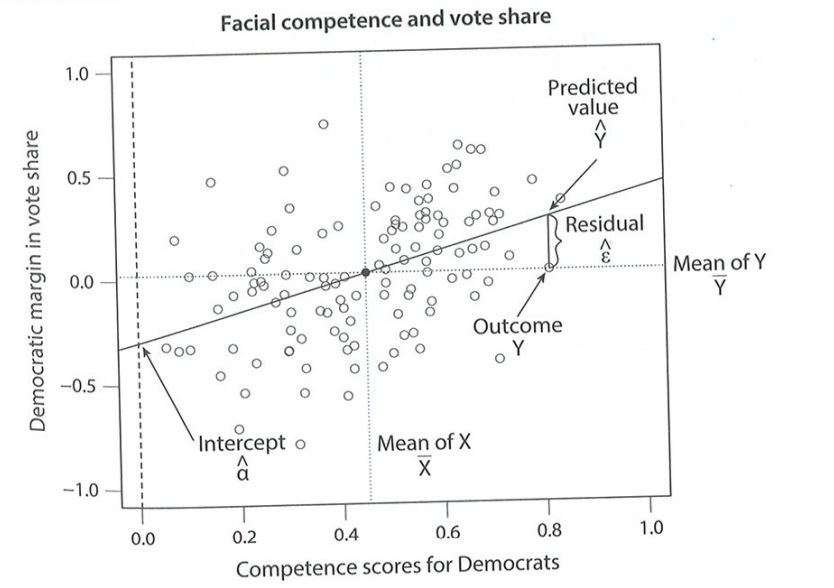
\includegraphics[scale=0.70]{reg_imai.png}
\caption{}
\label{}
\end{figure}

\section*{R-square - the coefficient of determination}

How good is a model? The more of the variance in the outcome $Y$ and $X$ is explained by the predictor $X$, the best is the model. How can we measure it?

If you didn't have any information on the relationship of $X$ and $Y$, and you want to guess the value of $Y$, what would be a good guess? The mean of $Y$.

With a regression model, you can guess better than just the mean value. You can use the conditional values of $Y$ on $X$ -- $E[Y|X]$ to improve you guess.

The difference between this two guesses -- the plain $Y$ expected value and the conditional expected value on $X$ -- is exactly the variation of $Y$ explained by the model and is represented by the model sum os squares:

\[MSS = \sum_{i=1}^n (\hat Y - \bar Y)^2 \]

The total variation in $Y$ is the total sum of squares:

\[TSS = \sum_{i=1}^n (Y_i - \bar Y)^2 \]

and it can be divided into two parts, MSS and SSR, or into a part that is explained by the model and a part that it is not. Remember that the Squared Sum of Residuals (SSR) i:

\[SSR = \sum_{i=1}^n (Y_i - \hat Y)^2 \]

The coefficient of determination, $R^2$, is the answer to the fist question. It is a measure of mdoel fit and represents the portion of $Y$ explained by $X$. It can be calculated using the summations described above:

\[R^2 = \frac{MSS}{TSS} = \frac{TSS - SSR}{TSS} = 1 - \frac{SSR}{TSS}\]
 
\end{document}

